\documentclass[11pt]{article}
\usepackage{inputenc}
\usepackage{comment}
\usepackage{fontspec}
\usepackage{authblk}
\usepackage{graphicx}
\usepackage{fancyhdr}
\usepackage{amssymb}
\usepackage{amsmath}
\usepackage{gensymb}
\usepackage{float}
\usepackage{enumerate}
\usepackage{tocloft}
\usepackage{abstract}
\usepackage[hidelinks]{hyperref}
\usepackage{appendix}
\usepackage[dvipsnames, svgnames, x11names]{xcolor}
\usepackage{dirtree}
\usepackage{cite}
\usepackage{geometry}
\usepackage{makecell}
\usepackage{multirow}
\usepackage{graphicx}
\usepackage{float}
\usepackage{subfig}
\usepackage[ruled]{algorithm2e}
\usepackage{indentfirst}
\usepackage{unicode-math}
\usepackage{afterpage}
\usepackage{tikz}

% \setlength{\headheight}{16pt}

\usepackage{setspace}
\doublespacing

\setmainfont{Times New Roman}

\pagestyle{fancy}

\renewcommand\thesection{\arabic{section}}

\newcommand*{\rmd}{\mathop{}\!\mathrm{d}}
\newcommand*{\sgn}{\mathrm{sgn}}
\renewcommand{\cftsecleader}{\cftdotfill{\cftdotsep}}

\title{\vspace{-1.5cm} \huge Stock Volatility Forecasting and Word Features Selection --- Based On 10-K Corpus}

\author{
  \parbox{0.3\textwidth}{
    \centering WANG Zeyu
    \vspace{.25cm}
  }
  \parbox{0.3\textwidth}{
    \centering LIU Chang
    \vspace{.25cm}
  }
  \parbox{0.3\textwidth}{
    \centering TAN Huangao
    \vspace{.25cm}
  }
  \parbox{0.3\textwidth}{
    \centering LI Borui
  }
  \parbox{0.3\textwidth}{
    \centering ZHU Xinqi
  }
  \parbox{0.3\textwidth}{
    \centering GAO Yifeng
  }
}

\date{\today}

\setcounter{tocdepth}{2}
\setcounter{secnumdepth}{3}

\begin{document}

\maketitle
\thispagestyle{empty}
\setcounter{page}{0}

\begin{abstract}
  As a key indicator of the market risk, the stock volatility is an important evidence to support the investment portfolio. The traditional time series models such as GARCH models only rely on the volatility, but ignore the unstructured text data like companies' 10-K reports, which is also shown to be helpful in forecasting. However, due to the complexity of natural language and the evolving semantic patterns, it is still challenging to extract operable signals from the narration of natural language. Focusing on exploring the relation between the 10-K report and stock volatility, we apply Lasso regression, Ridge regression, and the decision tree on the companies' 10-K reports together with historical volatility, to predict the future volatility. The result shows that it can perform much better than the Naive model. Meanwhile, based on the word features given by the models, we also explore the difference of word features between the years and models and found it changes due to some big events.
  \\\\
  \textbf{Keywords:} Lasso; Ridge; decision tree; stock volatility; natural language processing.
\end{abstract}

\newpage

\section{Introduction}

\subsection{Motivation and Goal}

As a key property to measure market risk, stock volatility includes uncertainty and different expectations of investor for stock investment \cite{RePEc:eee:finlet:v:69:y:2024:i:pb:s1544612324011929}, which is important for portfolio \cite{ta2020portfolio}. In the internet era, the repidly growing unstructured text data, especially in the aspect of company disclosure, enables the model to rely more on unstructured text data like the reports or acts \cite{RAJENDRAN2024101813} rather than structed data like historical prices and volatility, which provides great potential for improve volatility prediction \cite{Ma2024} . Even though the previous research has preliminarily shown the link between text sentiment and short-term market response \cite{li2022sentiment}, it is still challenging to extract operable signals from the narration of natural language due to the complexity of natural language and the evolving semantic patterns in the annual report.

Based on the above motivation, we hope to predict the logarithmic volatility of stock returns in the next year by studying the MD\&A part of the form 10-K report \cite{MATTERA20241539}\cite{ma2023stock}, as well as identify and evaluate the importance of a single token in volatility prediction. The machine learning model including Lasso/Ridge regression and decision tree, combining with the NLP technology \cite{yogatama2015sparse} will be used to establish the framework for text driven volatility prediction, reveal language patterns, and provide effective information for investment strategies, company disclosures and regulatory practices.

\subsection{Datasets}

The 10-K Corpus \cite{kogan2009predicting} is a widely used dataset including the 10-K reports from thousands of companies, with the stock return volatility measurements in the one year period before and after each report. Its subset is used in our work, including the log volatility (e.g., 1996.logvol.-12.txt), as well as the tokenized MD\&A sections (e.g., 1996.tok.tgz), which provides us with the detailed discussion about the operations of the company and some forward looking statements \cite{brown2024financial}. As for the other data, such as the meta data about the companies, are regarded irrelevant to our goals.

\section{Methods}

\subsection{Text preprocessing}

We use the Natural Language Toolkit (NLTK) \cite{nltk-py} as lemmatizer, stemmer and stop token filter with the idea that: (1) Some words including articles, prepositions and conjunctions are regarded as insignificant in text analysis but appears in every report; (2) Words appear in several inflected forms but with same meaning should be considered as the same, and should be transformed to their stem, so that they can be clustered together. Through these text preprocessing method, we can greatly reduce the text volume, eliminate the noise, and improve the efficiency of the following steps.

\subsection{Term Frequency–Inverse Document Frequency (TF-IDF)}

The term frequency–inverse focument frequency (TF-IDF) \cite{sparck1972statistical}\cite{robertson2004understanding} measures the importance of a word to a document in corpus via

$$
  \begin{aligned}
     & \text{(Term frequency)}             & \mathrm{tf}(t, d)  & = \frac{f_{t, d}}{\sum_{t^\prime \in d} f_{t^\prime, d}},                                     \\
     & \text{(Inverse document frequency)} & \mathrm{idf}(t, d) & = \log_2\left( \frac{N}{\left\vert \left\{ d: d \in D, t \in d \right\} \right\vert} \right),
  \end{aligned}
$$

where $f_{t, d}$ is the raw count of a term $t$ in a document $d$, and $N$ is the total number of documents. With the TF-IDF, each company's 10-K report is represented by a vector that highlights discriminative keywords.

\subsection{Nonnegative Matrix Factorization (NMF)}

In order to further reduce the dimension of the input data, we use the nonnegative matrix factorization (NMF) \cite{lee2000algorithms}, with which we can decomposes the TF-IDF matrix $X \in \mathbb{R}^{n \times m}$ into two nonnegative smaller matrices $W \in \mathbb{R}^{n \times d}$ and $H \in \mathbb{R}^{d \times m}$, where $X \approx W H$ and $d$ is the given number of dimension.

The previous research \cite{lee1999learning} have shown that this method is particularly suitable for text data due to non-negativity and is able to learn the semantic features of text, which allows us to extract interpretable latent topics that capture the underlying themes in the MD\&A sections. Besides, unlike other dimensionality reduction techniques like PCA, NMF provides sparse and parts-based representations, making it easier to identify meaningful topics and understand the contribution of individual words.

\subsection{Naive Model (Baseline)}

The previous research \cite{beck2025mind} has shown that the naive model is better than many other complex models, especially for high-volatility time series. Thus we choose the naive model (or Persistence model) as our baseline, which uses the current (or same period) value as the forecast. Since it only requires the  doesn't involve the word features or any assumptions.

\subsection{Lasso/Ridge Regression \& Decision Tree}

The models we used are Lasso regression, Ridge regression and Decision Tree, which are all widely known. These models (also their extensions) are powerful in forecast and can have better performance compare with other models like heterogeneous autoregressive (HAR) models \cite{liang2023forecasting} \cite{li2022forecasting} \cite{christensen2023machine}. In addition, they are well-known inherently interpretable, which can help us extract whether a word implies the increasing or decreasing of volatility.

\subsection{Model Evaluation}

The two widely used measurement MAE and MSE will be used to evaluate the results. Given the prediction $\hat{x}$ and ground truth $x$, they are computed as

$$
  \text{MAE}(x, \hat{x}) = \frac{1}{N} \sum_{i=1}^N \vert x_i - \hat{x}_i \vert,\quad \text{MSE}(x, \hat{x}) = \frac{1}{N} \sum_{i=1}^N  (x_i - \hat{x}_i)^2. \\
$$

Another problem we are interested in is the words features. We first compute the weight of each words via the pseudo inverse of $H$ with $H^+ \beta = (V^T \Lambda^+ U) \beta$, where $\beta \in \mathbb{R}^d$ is the model parameter and $H \in \mathbb{R}^{d \times m}$ is components by NMF. Here the pseudo inverse $H^+$ is calculate from the SVD that $H = U^T \Lambda V$, and $\Lambda^+$ is the diagonal matrix consisting of the reciprocals of $H$'s singular values. In order to compare the features cross models and years, we selected the top $1000$ words (about $1\% \sim 5\%$ of total) for each model and check whether they are similar between different methods and years.

\subsection{Overview}

\begin{figure}[H]
  \centering
  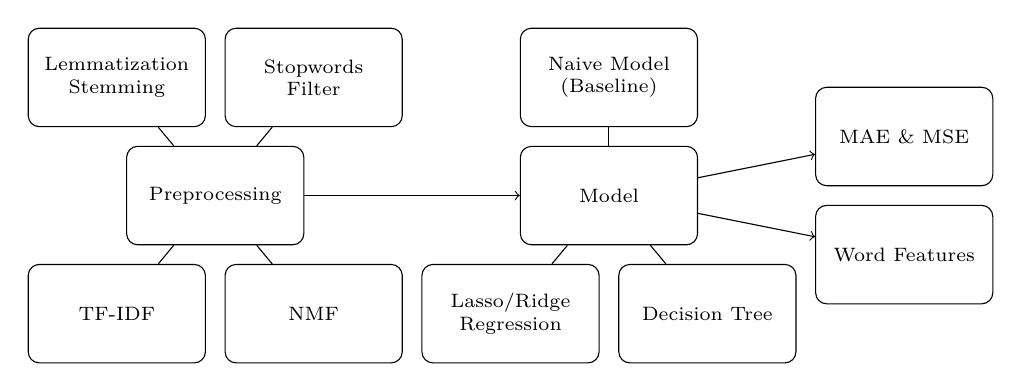
\begin{tikzpicture}[minimum width=2.25cm, minimum height=1.25cm, font=\scriptsize]
    \node[draw, align=center, rounded corners]  (P)   at ( 0.00,  0.00)   {Preprocessing};
    \node[draw, align=center, rounded corners]  (LS)  at (-1.25,  1.50)   {Lemmatization \\ Stemming};
    \node[draw, align=center, rounded corners]  (SF)  at ( 1.25,  1.50)   {Stopwords \\ Filter};
    \node[draw, align=center, rounded corners]  (T)   at (-1.25, -1.50)   {TF-IDF};
    \node[draw, align=center, rounded corners]  (N)   at ( 1.25, -1.50)   {NMF};

    \node[draw, align=center, rounded corners]  (M)   at ( 5.00,  0.00)   {Model};
    \node[draw, align=center, rounded corners]  (NM)  at ( 5.00,  1.50)   {Naive Model \\ (Baseline)};
    \node[draw, align=center, rounded corners]  (LR)  at ( 3.75, -1.50)   {Lasso/Ridge \\ Regression};
    \node[draw, align=center, rounded corners]  (D)   at ( 6.25, -1.50)   {Decision Tree};

    \node[draw, align=center, rounded corners]  (E)   at ( 8.75,  0.75)   {MAE \& MSE};
    \node[draw, align=center, rounded corners]  (W)   at ( 8.75, -0.75)   {Word Features};

    \draw[->] (P) -- (M);

    \draw[-] (P) -- (LS);
    \draw[-] (P) -- (SF);
    \draw[-] (P) -- (T);
    \draw[-] (P) -- (N);

    \draw[-] (M) -- (NM);
    \draw[-] (M) -- (LR);
    \draw[-] (M) -- (D);

    \draw[->] (M) -- (E);
    \draw[->] (M) -- (W);
  \end{tikzpicture}
  \caption{Overview flowchart for our method.}
  \label{figure-flowchart}
\end{figure}

The Figure \ref{figure-flowchart} is an overview of our method. The number of the components by NMF is set to $20$ balancing the memory, time and the accuracy. Consider the number that coefficients close to zero and the model error, the penalty is $0.00005$ for Lasso and $1.0$ for Ridge, meanwhile, the depth of the tree is set to $5$.

Then we test the model in two approaches. First we choose the data from one or several years, and split them into training dataset ($80\%$) and test dataset ($20\%$). In this case, the model is trained and tested on the data from same years, thus to avoid the flukes cause by splitting, we repeat the experiment for $400$ times, with the central limit theorem and sample variance, we can control the error under $0.003$ (with the probability over $95\%$), which is accurate enough.

Another test is to train the model via the data from one or several years and forecast the following year. In this case, we use all the data from previous years as the training set and the whole following year's data as the testing set. This approach will be run once to show the model's ability to deal with the new text data.

\section{Result}

\subsection{Forecasting error}

\subsubsection{Error with 1-year's training data}

We first train the data with 1-year text data and volatility. The Figure \ref{figure-1-year-test} shows the error of the model predicting the volatility in the same year, while the Figure \ref{figure-1-year-pred} shows the error of the prediction with the text and volatility of the next year.

\afterpage{
  \clearpage
  \begin{figure}[H]
    \centering
    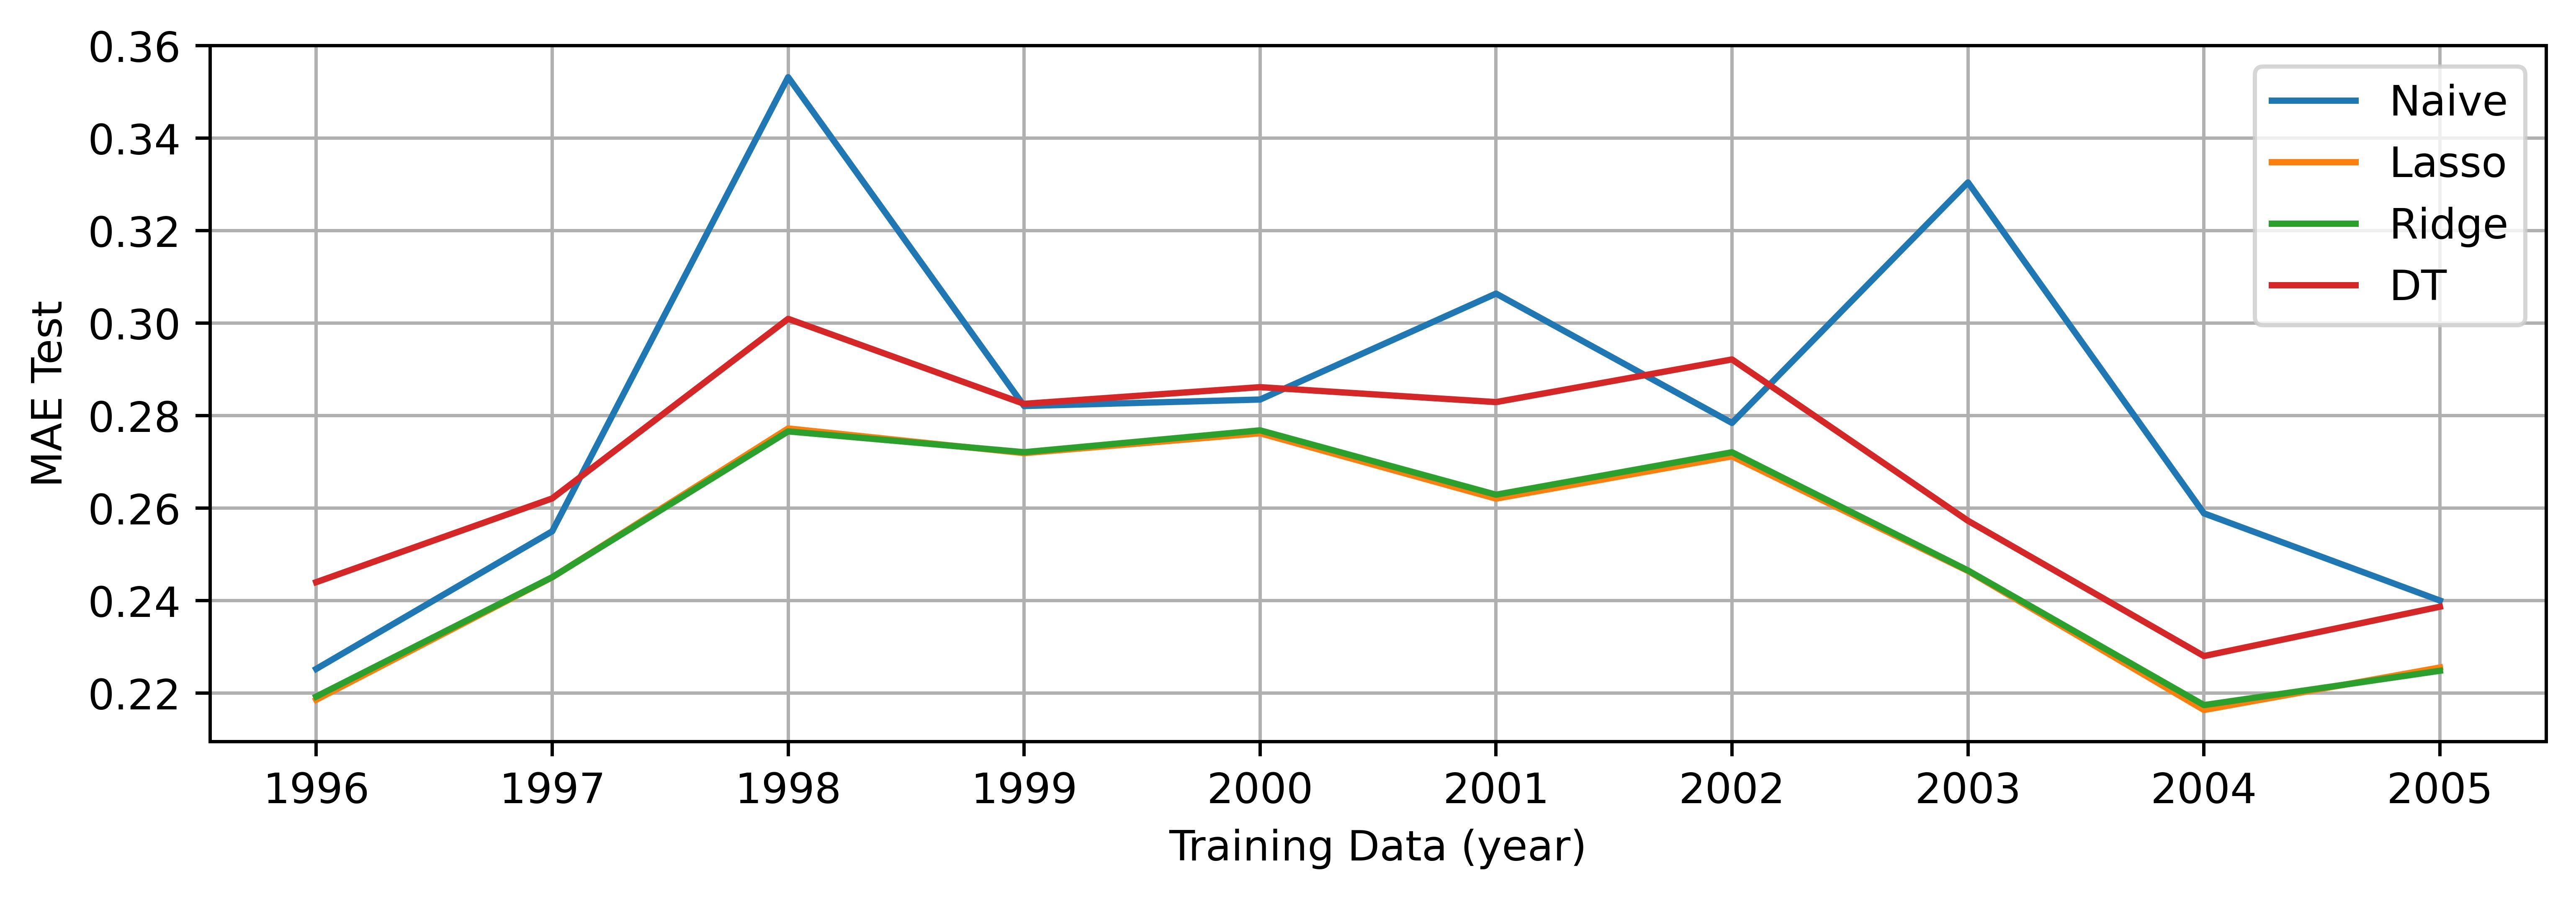
\includegraphics[width=0.7\textwidth]{../Result/Res-1_MAE_test.jpg} \\
    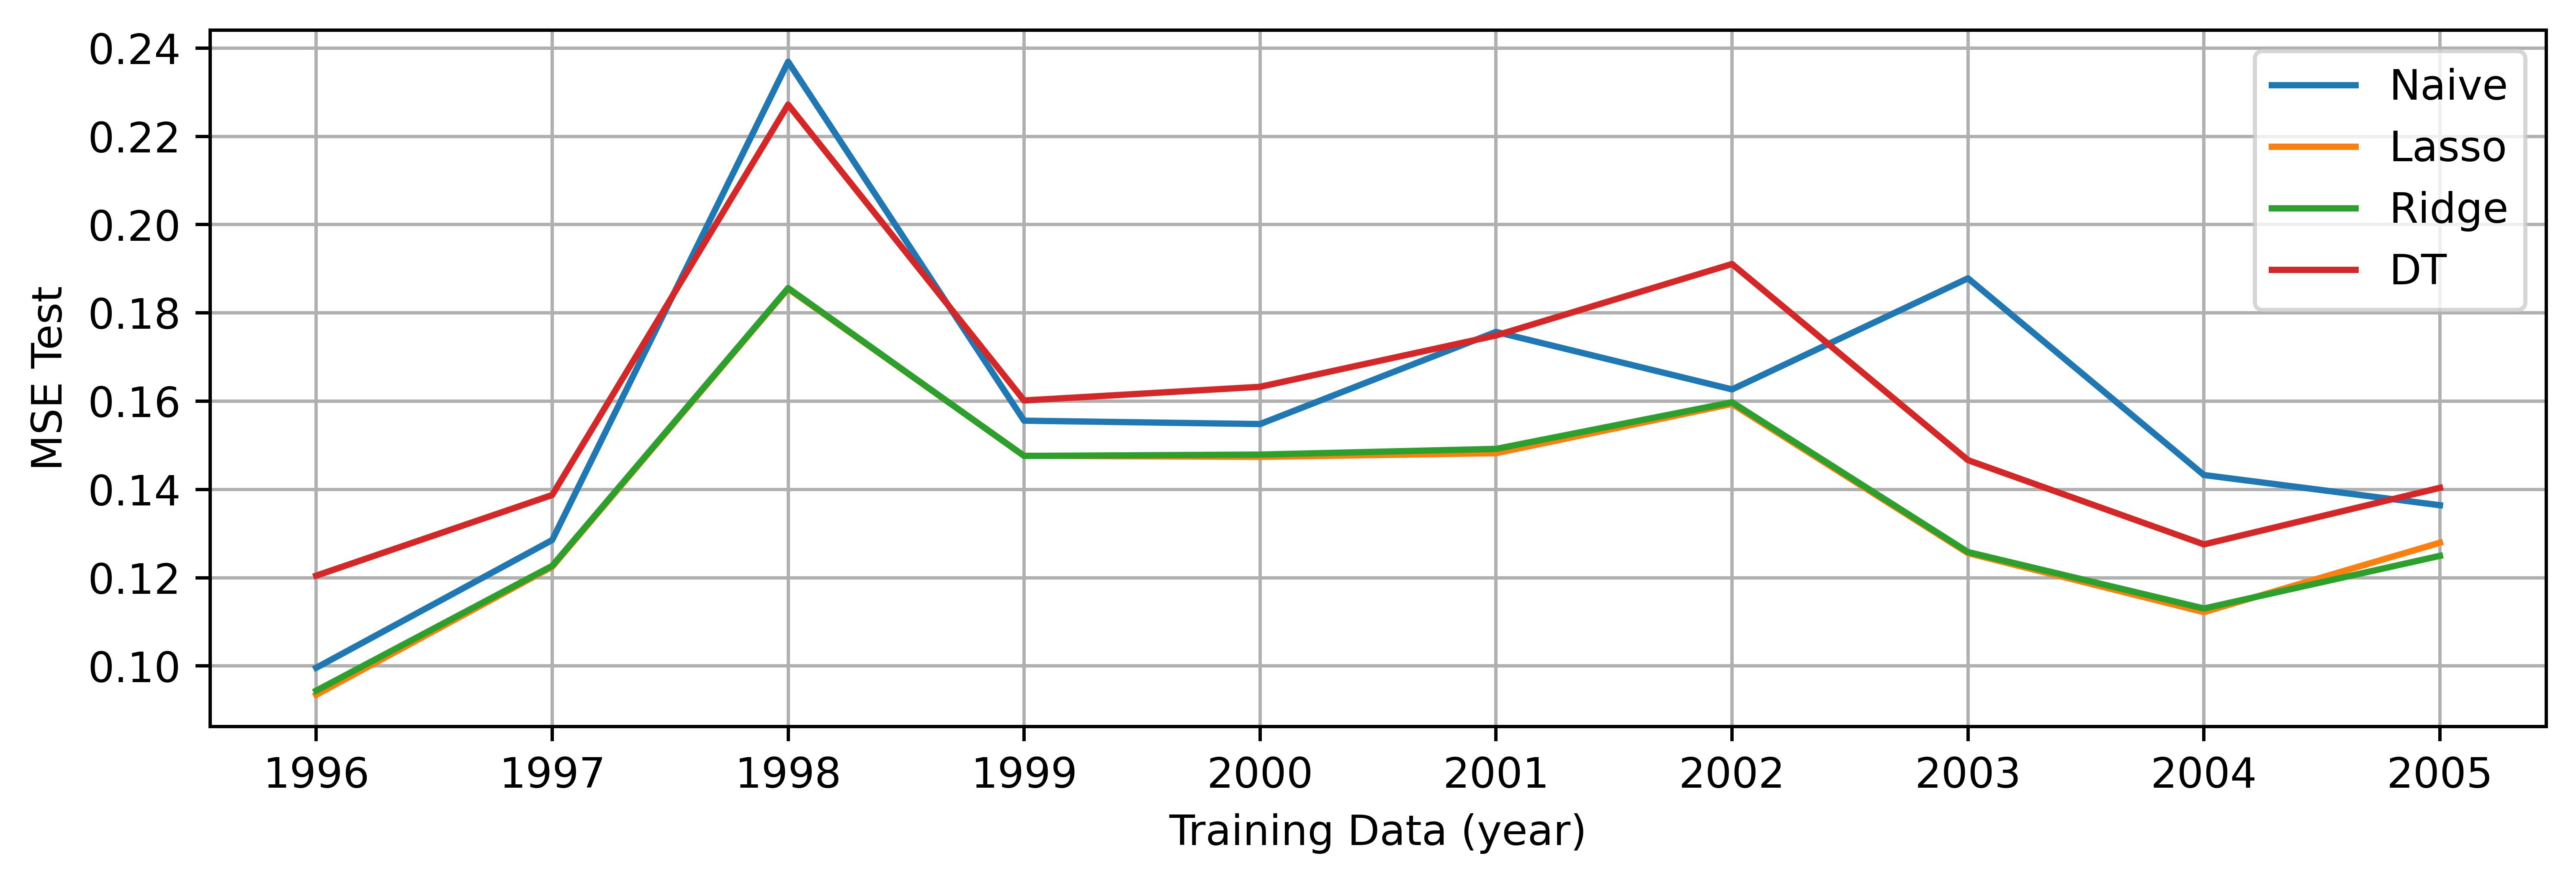
\includegraphics[width=0.7\textwidth]{../Result/Res-1_MSE_test.jpg}
    \caption{MAE and MSE for predicting the 1-year's data with the model trained by the same 1-year's data.}
    \label{figure-1-year-test}
  \end{figure}

  \begin{figure}[H]
    \centering
    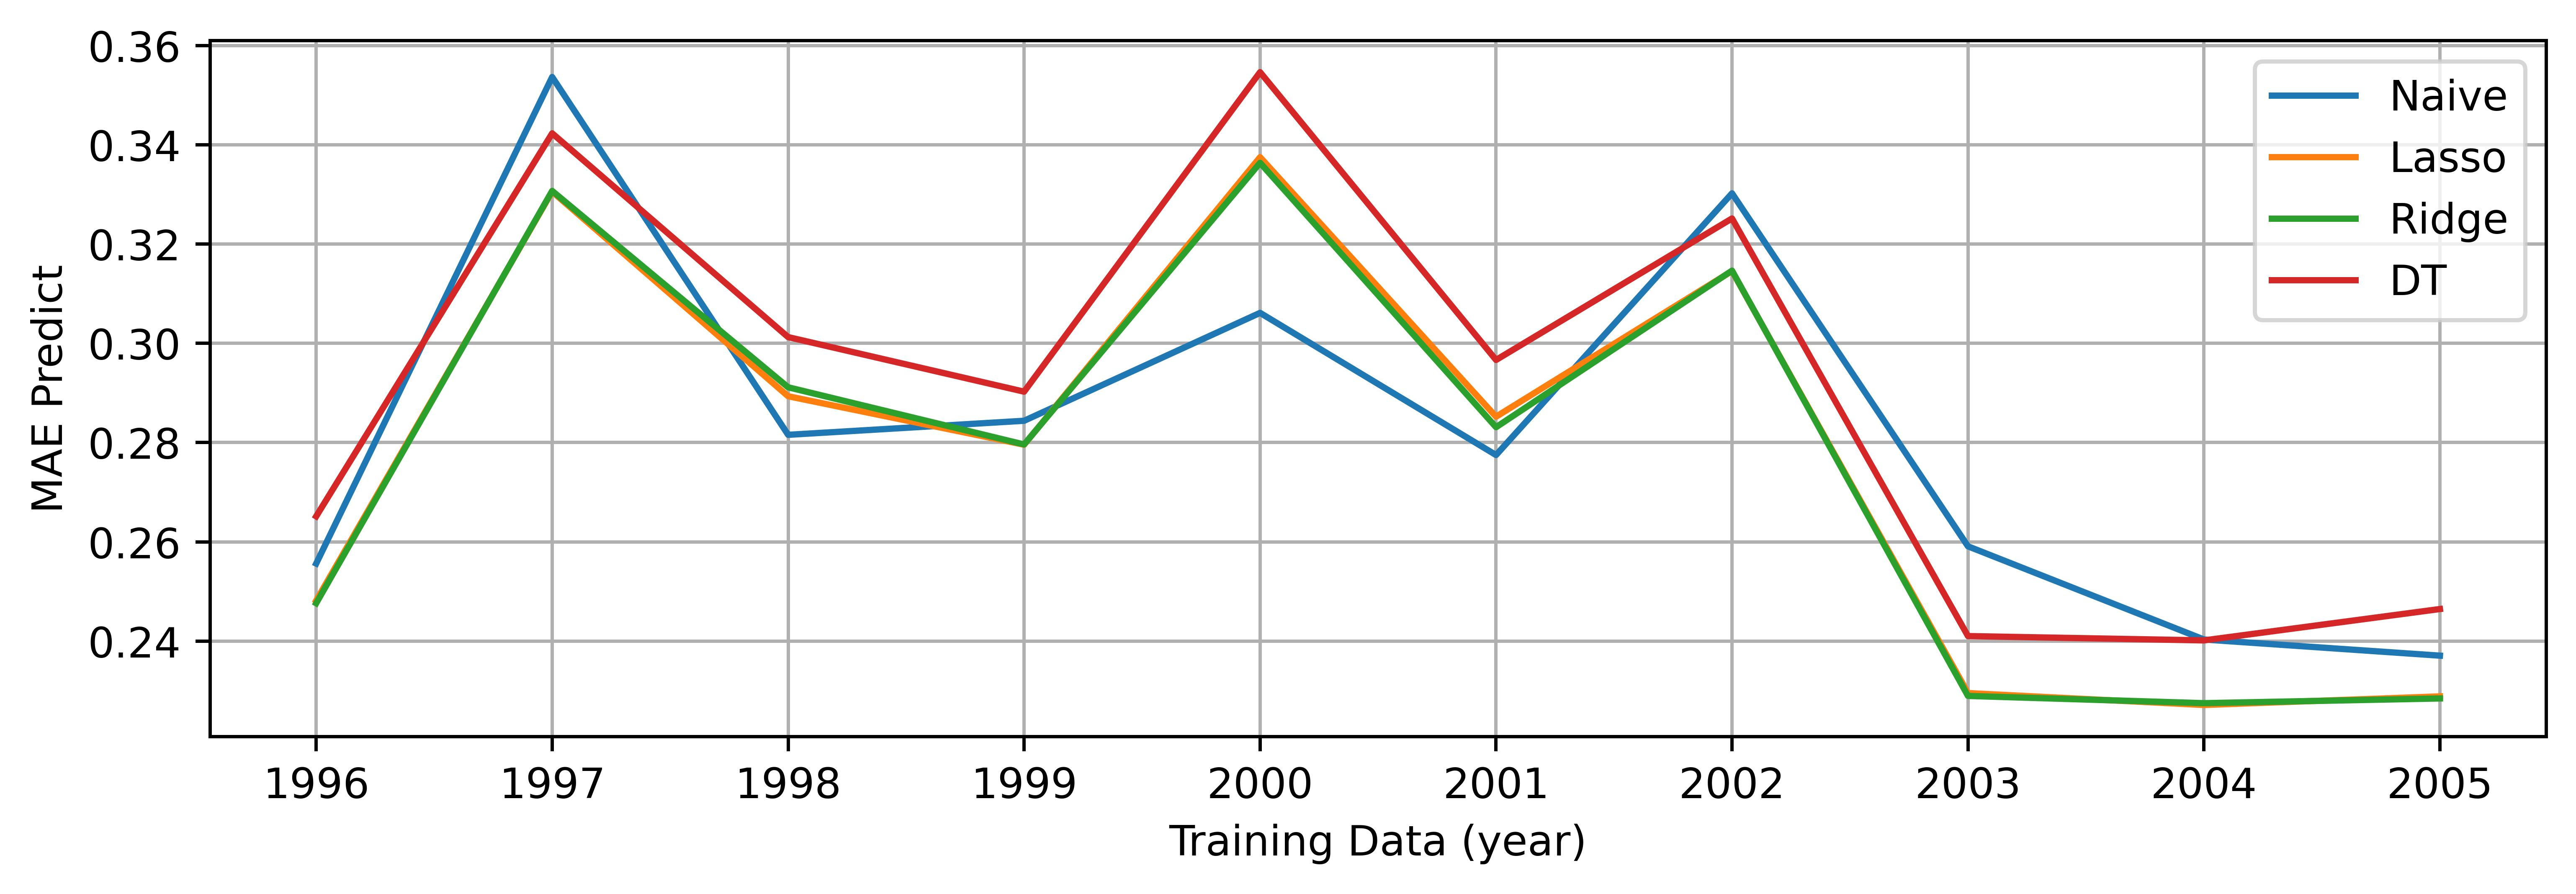
\includegraphics[width=0.7\textwidth]{../Result/Res-1_MAE_pred.jpg} \\
    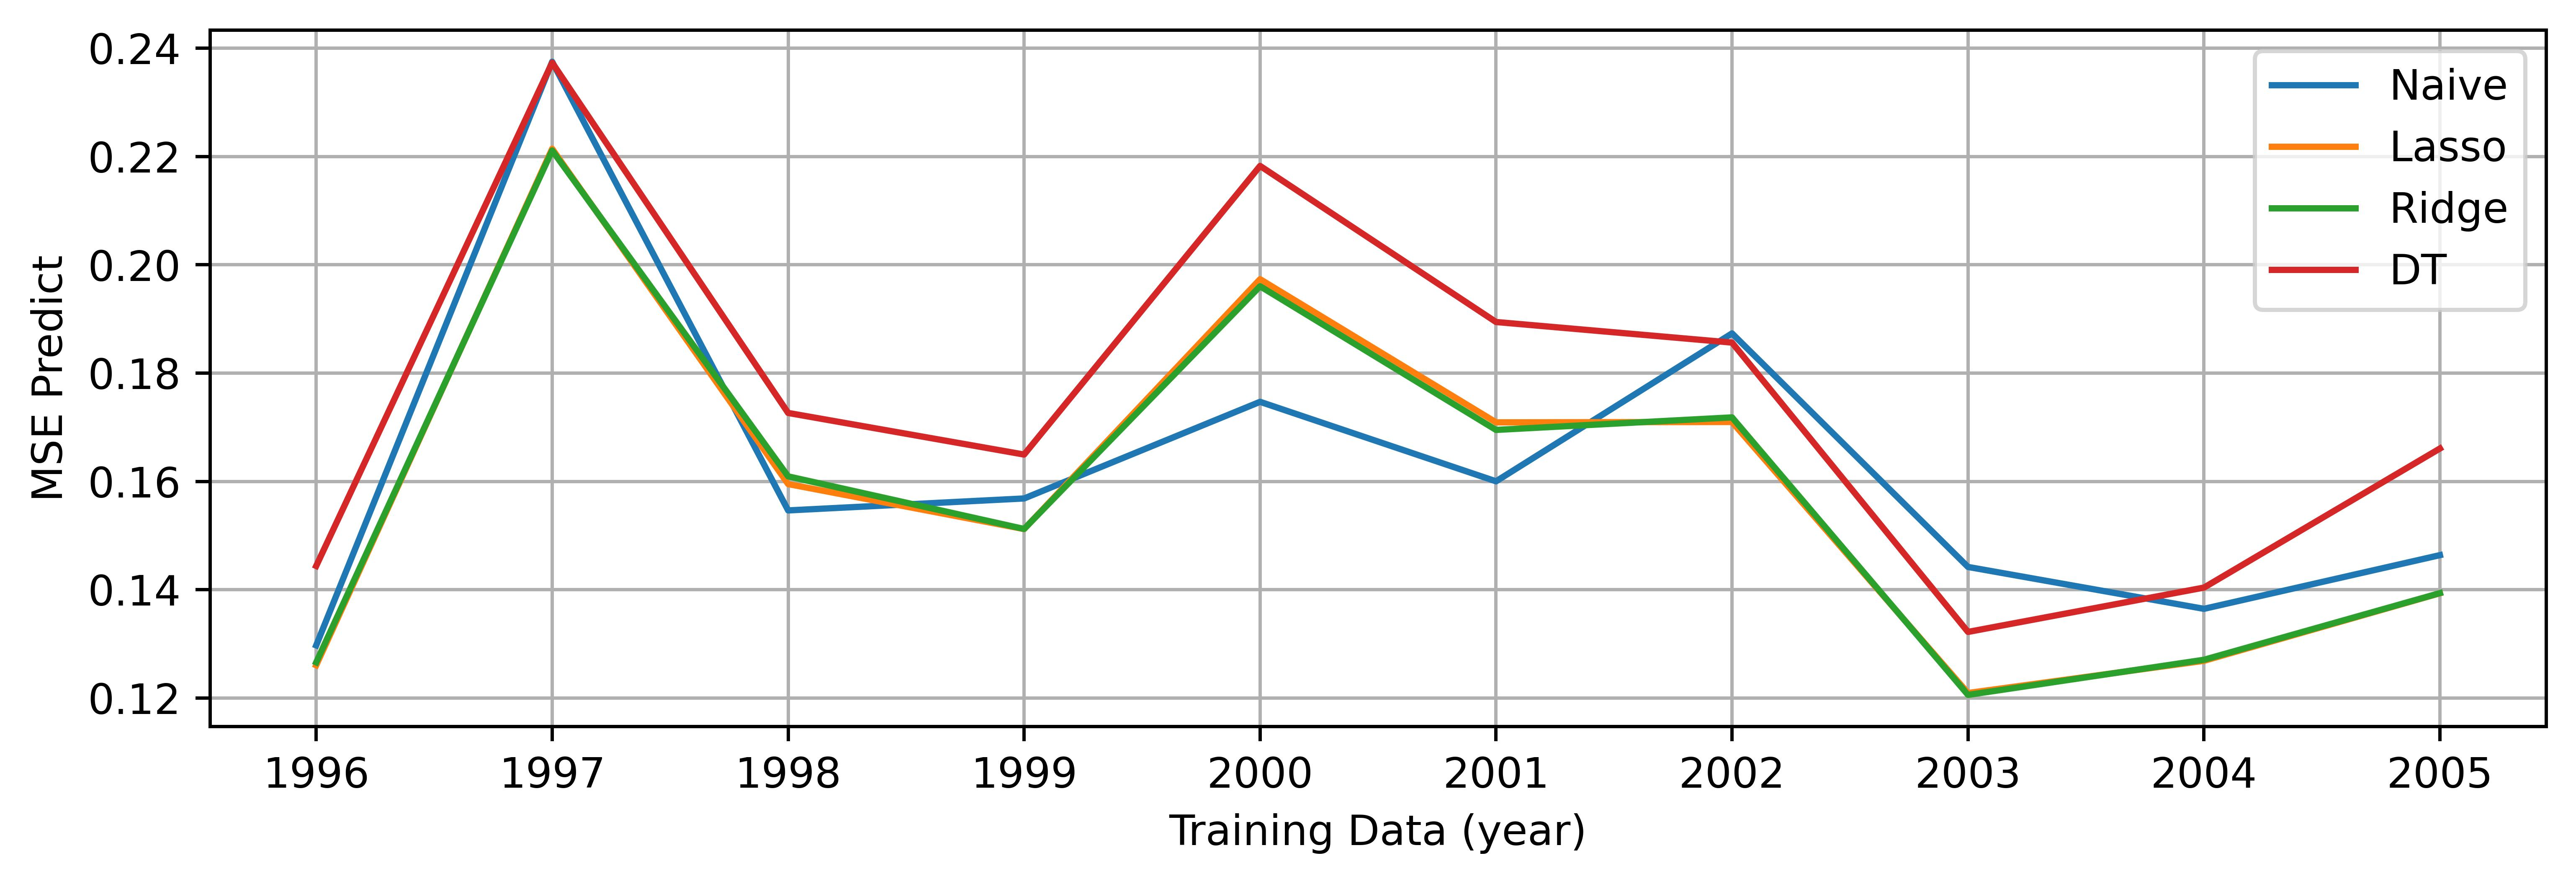
\includegraphics[width=0.7\textwidth]{../Result/Res-1_MSE_pred.jpg}
    \caption{MAE and MSE for predicting the following 1-year's data with the model trained by the previous 1-year's data.}
    \label{figure-1-year-pred}
  \end{figure}
  \clearpage
}

From the result, we can infer that the Lasso and Ridge regression can get almost the same error while the error of the decision tree is much higher. And all the models perform better when predicting the volatility of the same year rather than the following year. Furthermore, the prediction of the following year's volatility, especially the result of Lasso and Ridge regression, achieves much more accurate after 2002 with the enforcement of Sarbanes-Oxley Act, which implies that the this act might make the report more informative. Another noticeable difference is the error of predicting the following years' volatility gets higher in 2000, which may cause by the dot-com bubble.

\subsubsection{Error with 3-years' training data}

It is widely known that more training data can lead to a better method performance, with the assumption that the data are from the same distribution. In this case, we presume that the information or the distribution of the words are similar across the nearby years. This assumption is reasonable, otherwise we can't expect the model to do the prediction. But it still needs to be certified.

Therefore we train the model with the data from nearby 3 year, and test the model on the same 3 year's data as well as the following year's data. The Figure \ref{figure-3-year-test} shows the error of the model predicting the volatility in the same 3 years, while the Figure \ref{figure-3-year-pred} shows the error of the prediction with the text and volatility of the following year.

\afterpage{
  \clearpage
  \begin{figure}[H]
    \centering
    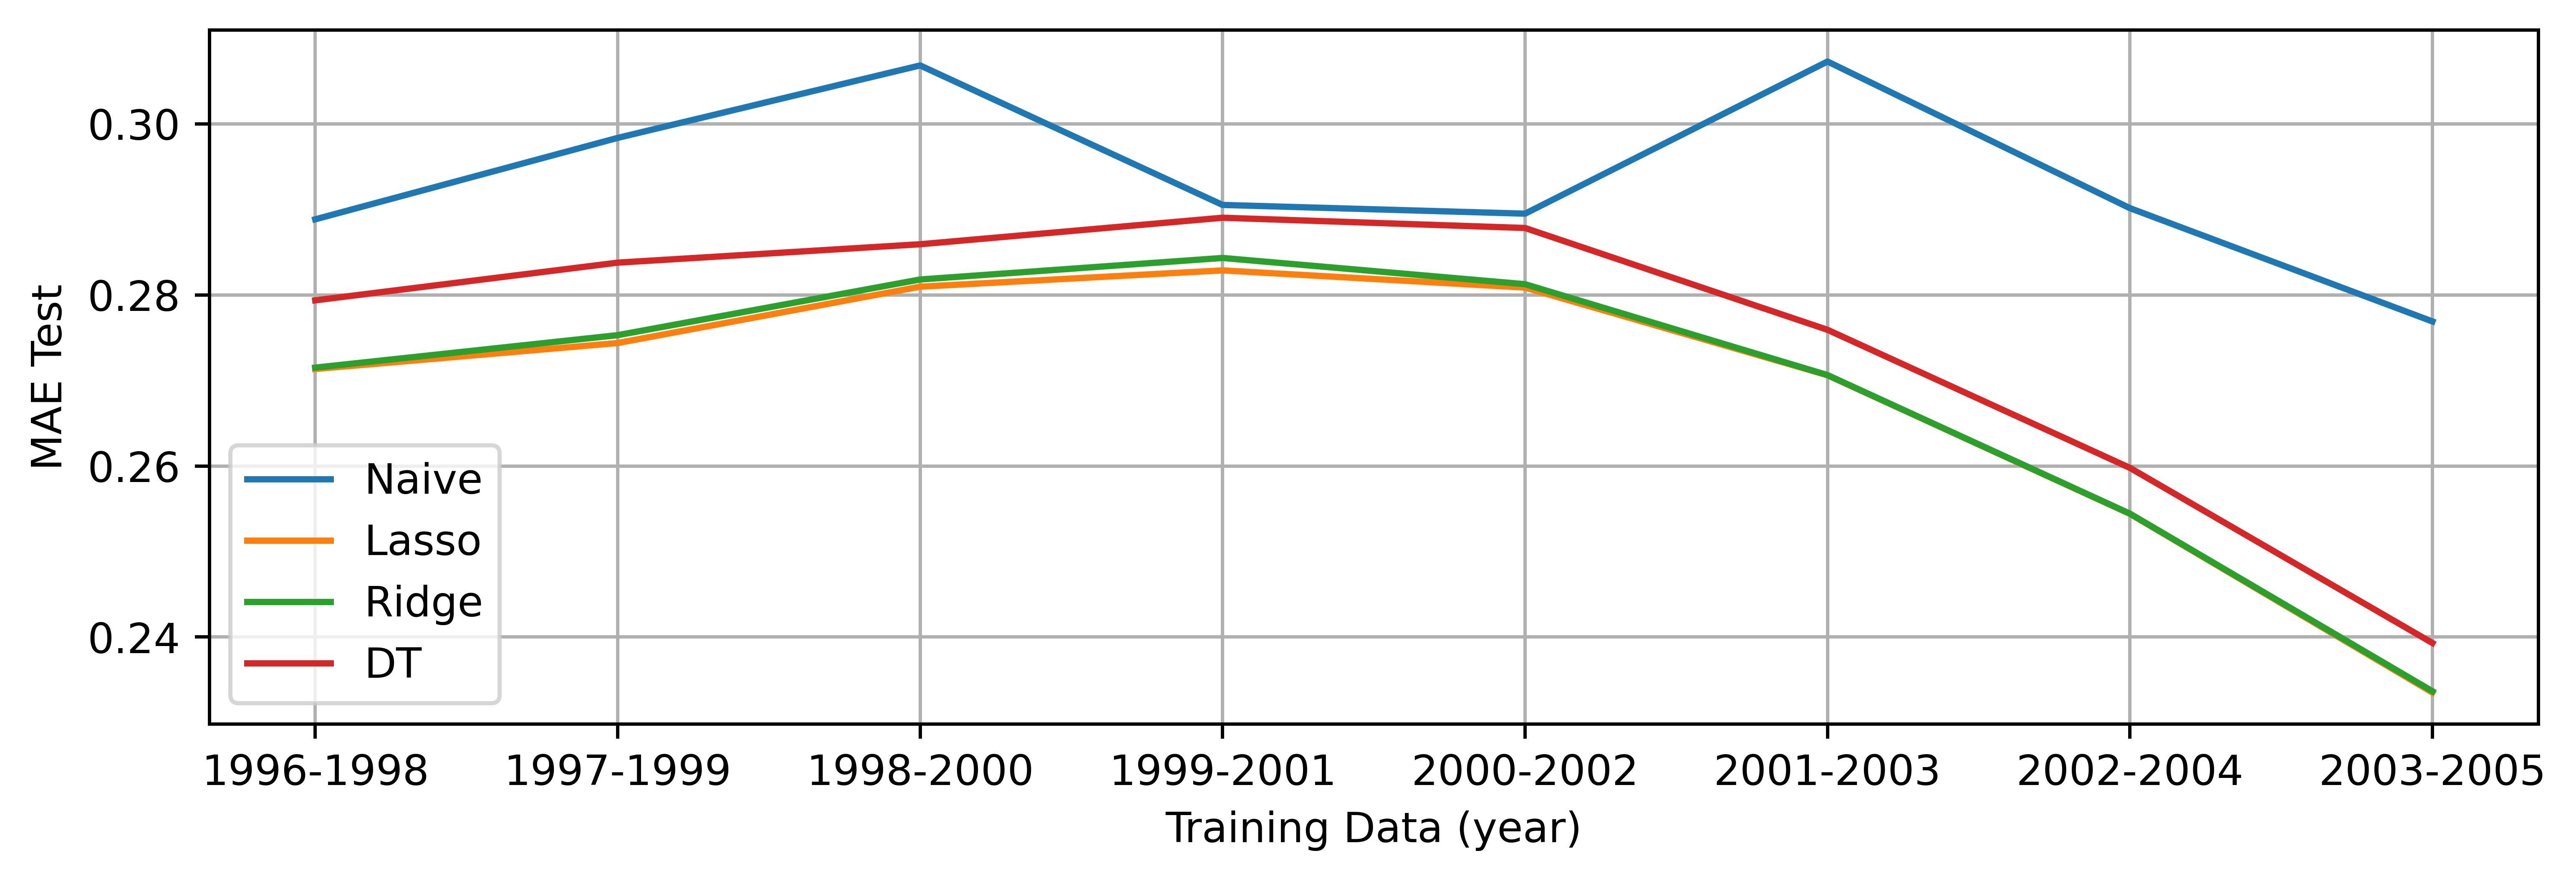
\includegraphics[width=0.7\textwidth]{../Result/Res-3_MAE_test.jpg} \\
    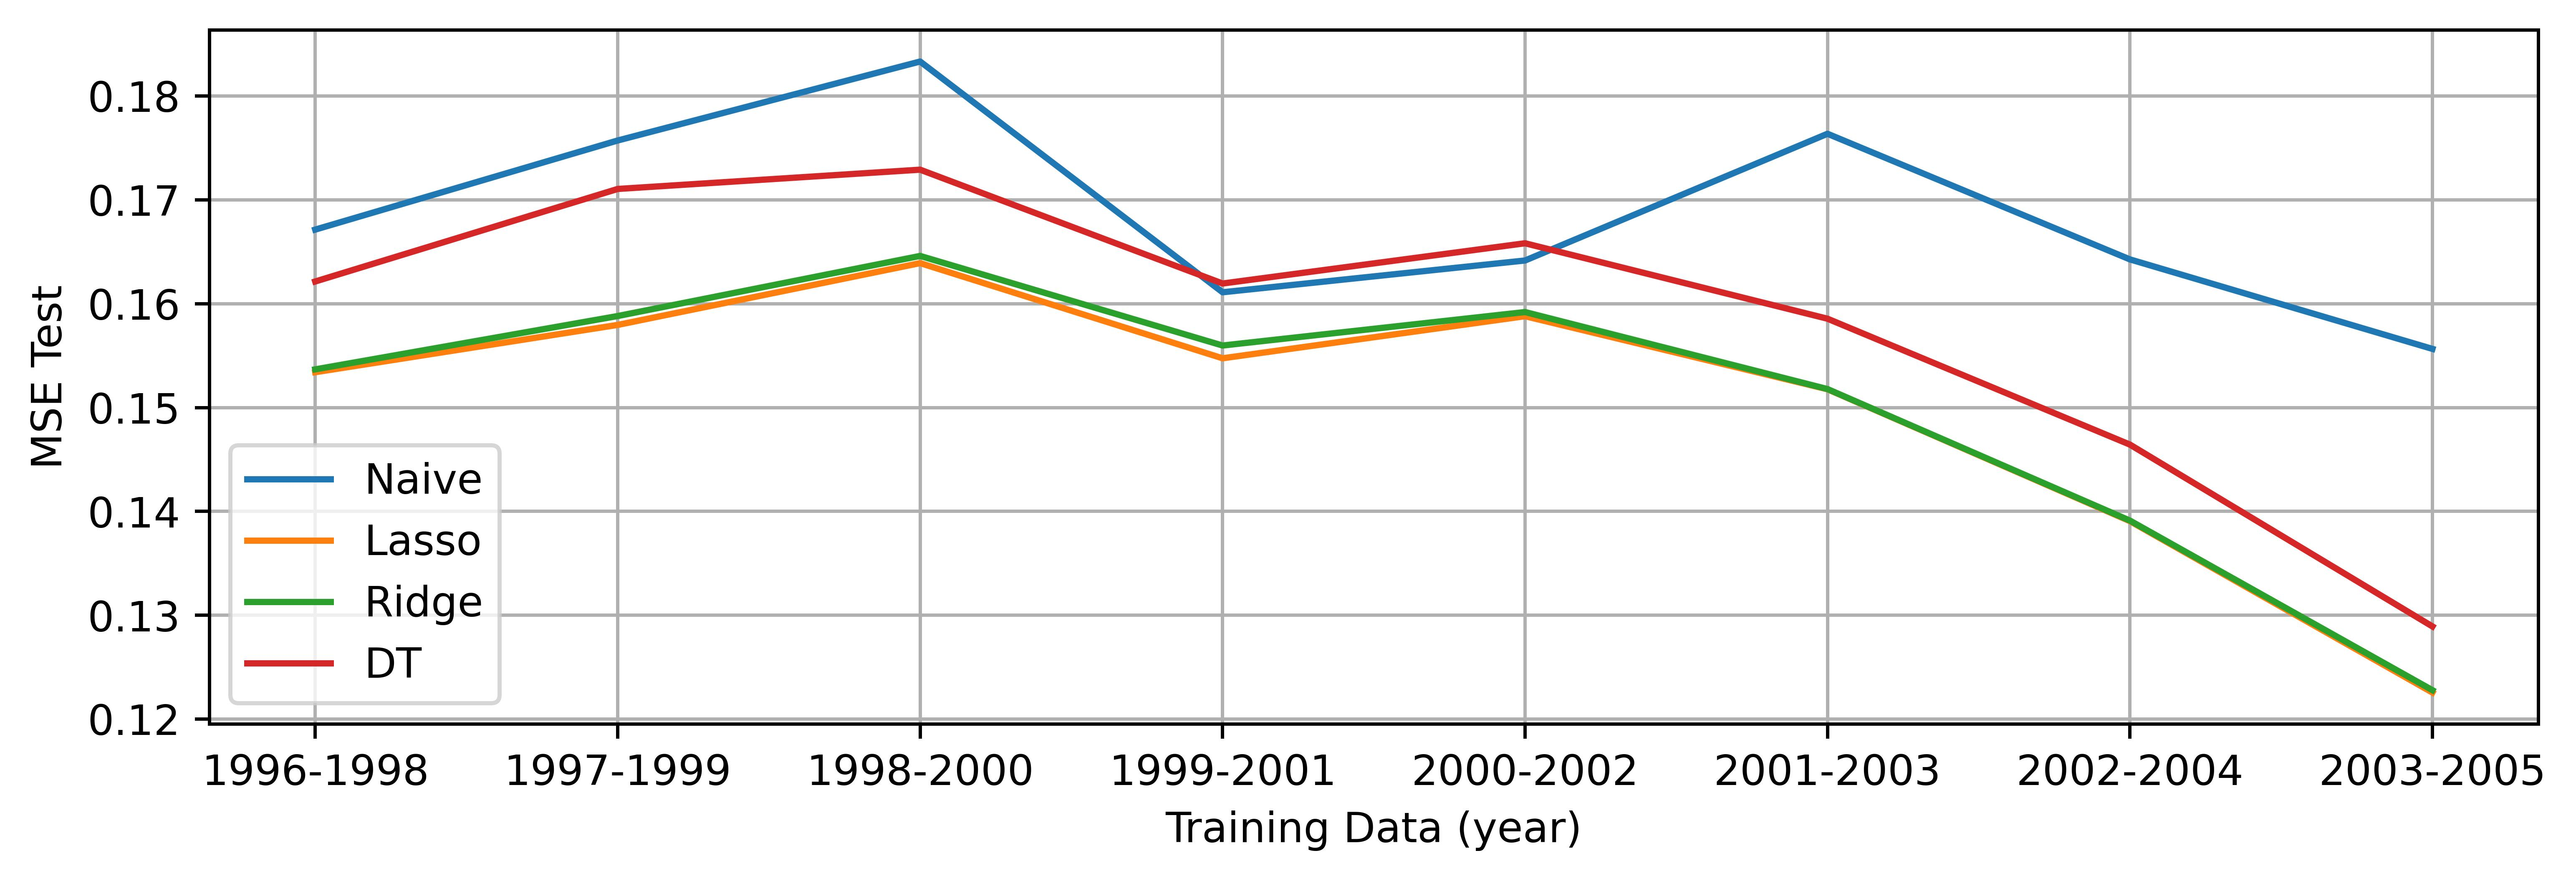
\includegraphics[width=0.7\textwidth]{../Result/Res-3_MSE_test.jpg}
    \caption{MAE and MSE for predicting the 3-years' data with the model trained by the same 3-years' data.}
    \label{figure-3-year-test}
  \end{figure}

  \begin{figure}[H]
    \centering
    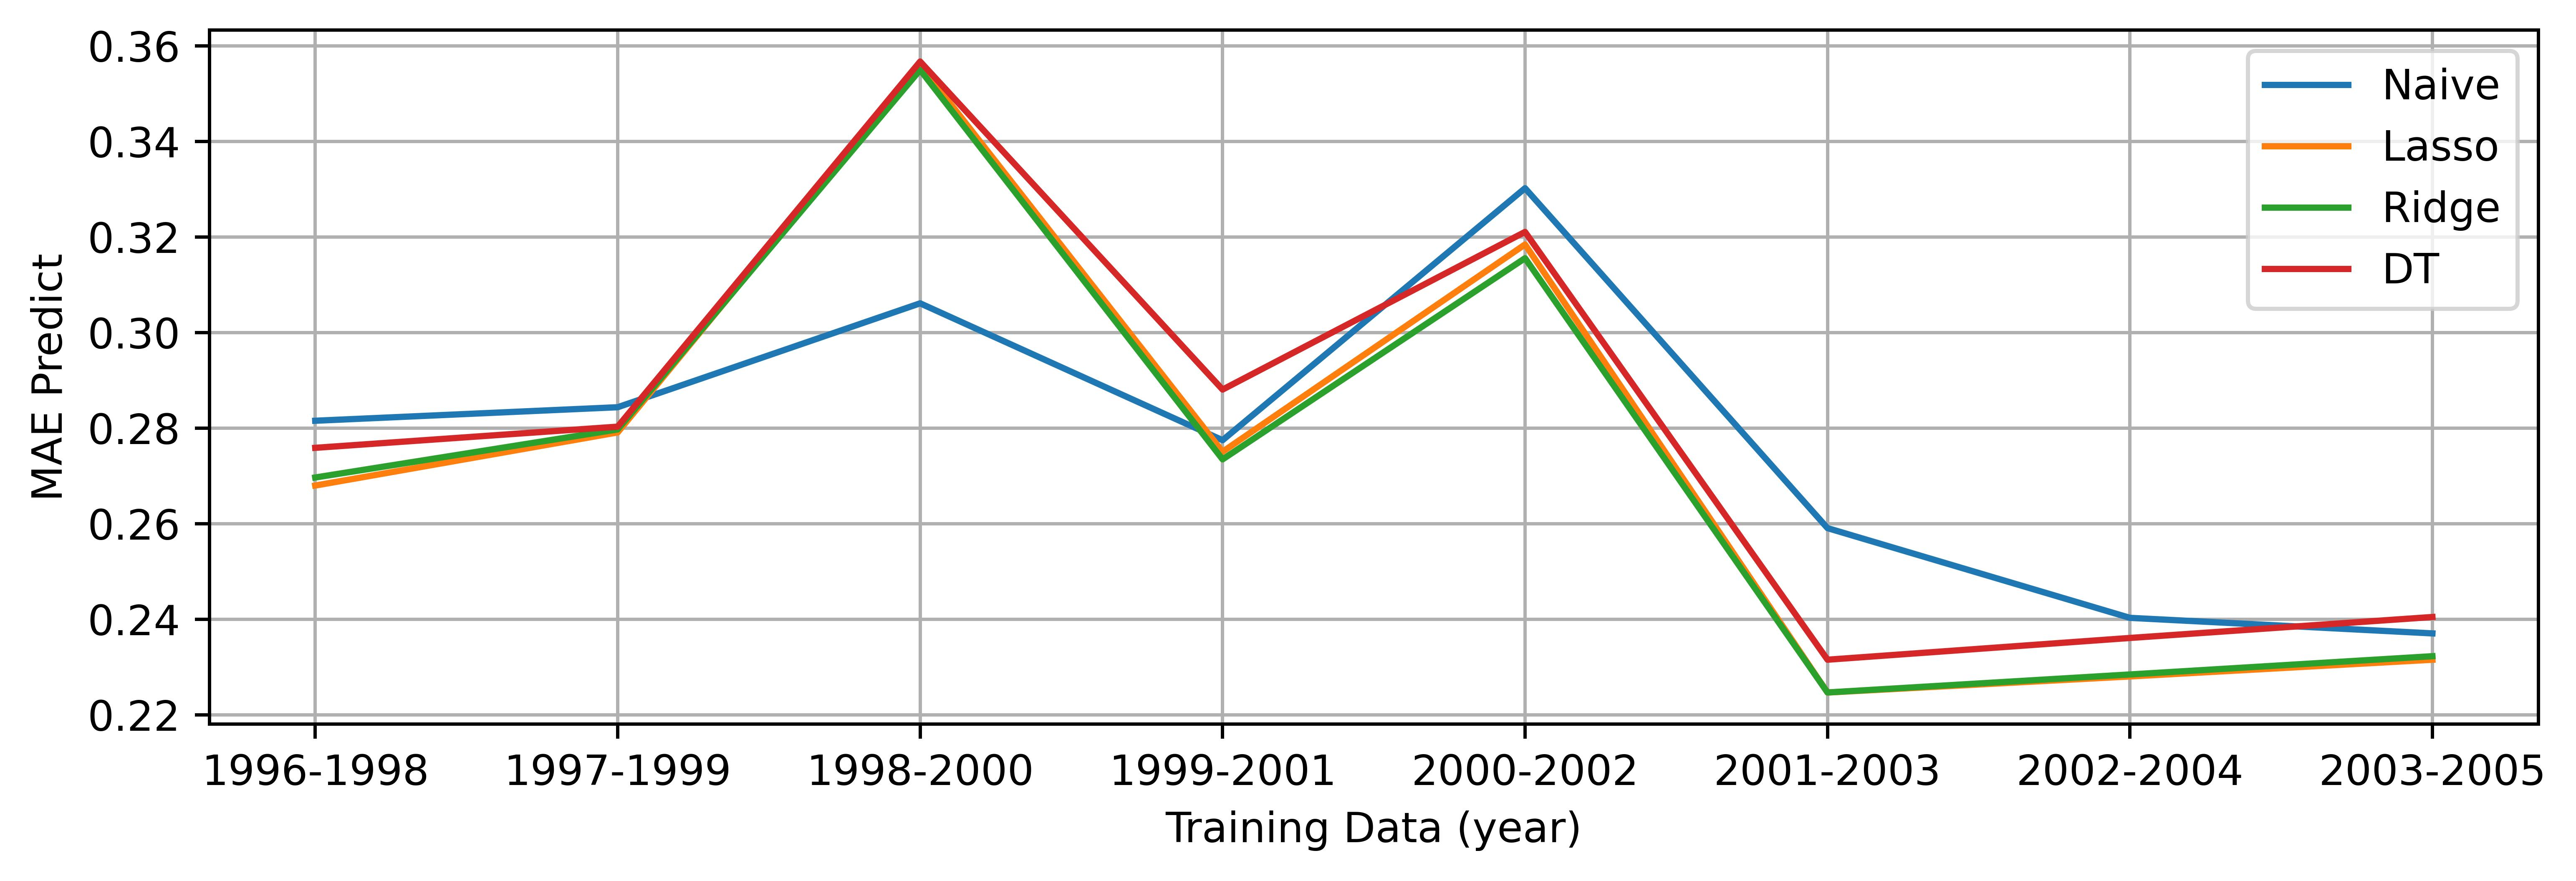
\includegraphics[width=0.7\textwidth]{../Result/Res-3_MAE_pred.jpg} \\
    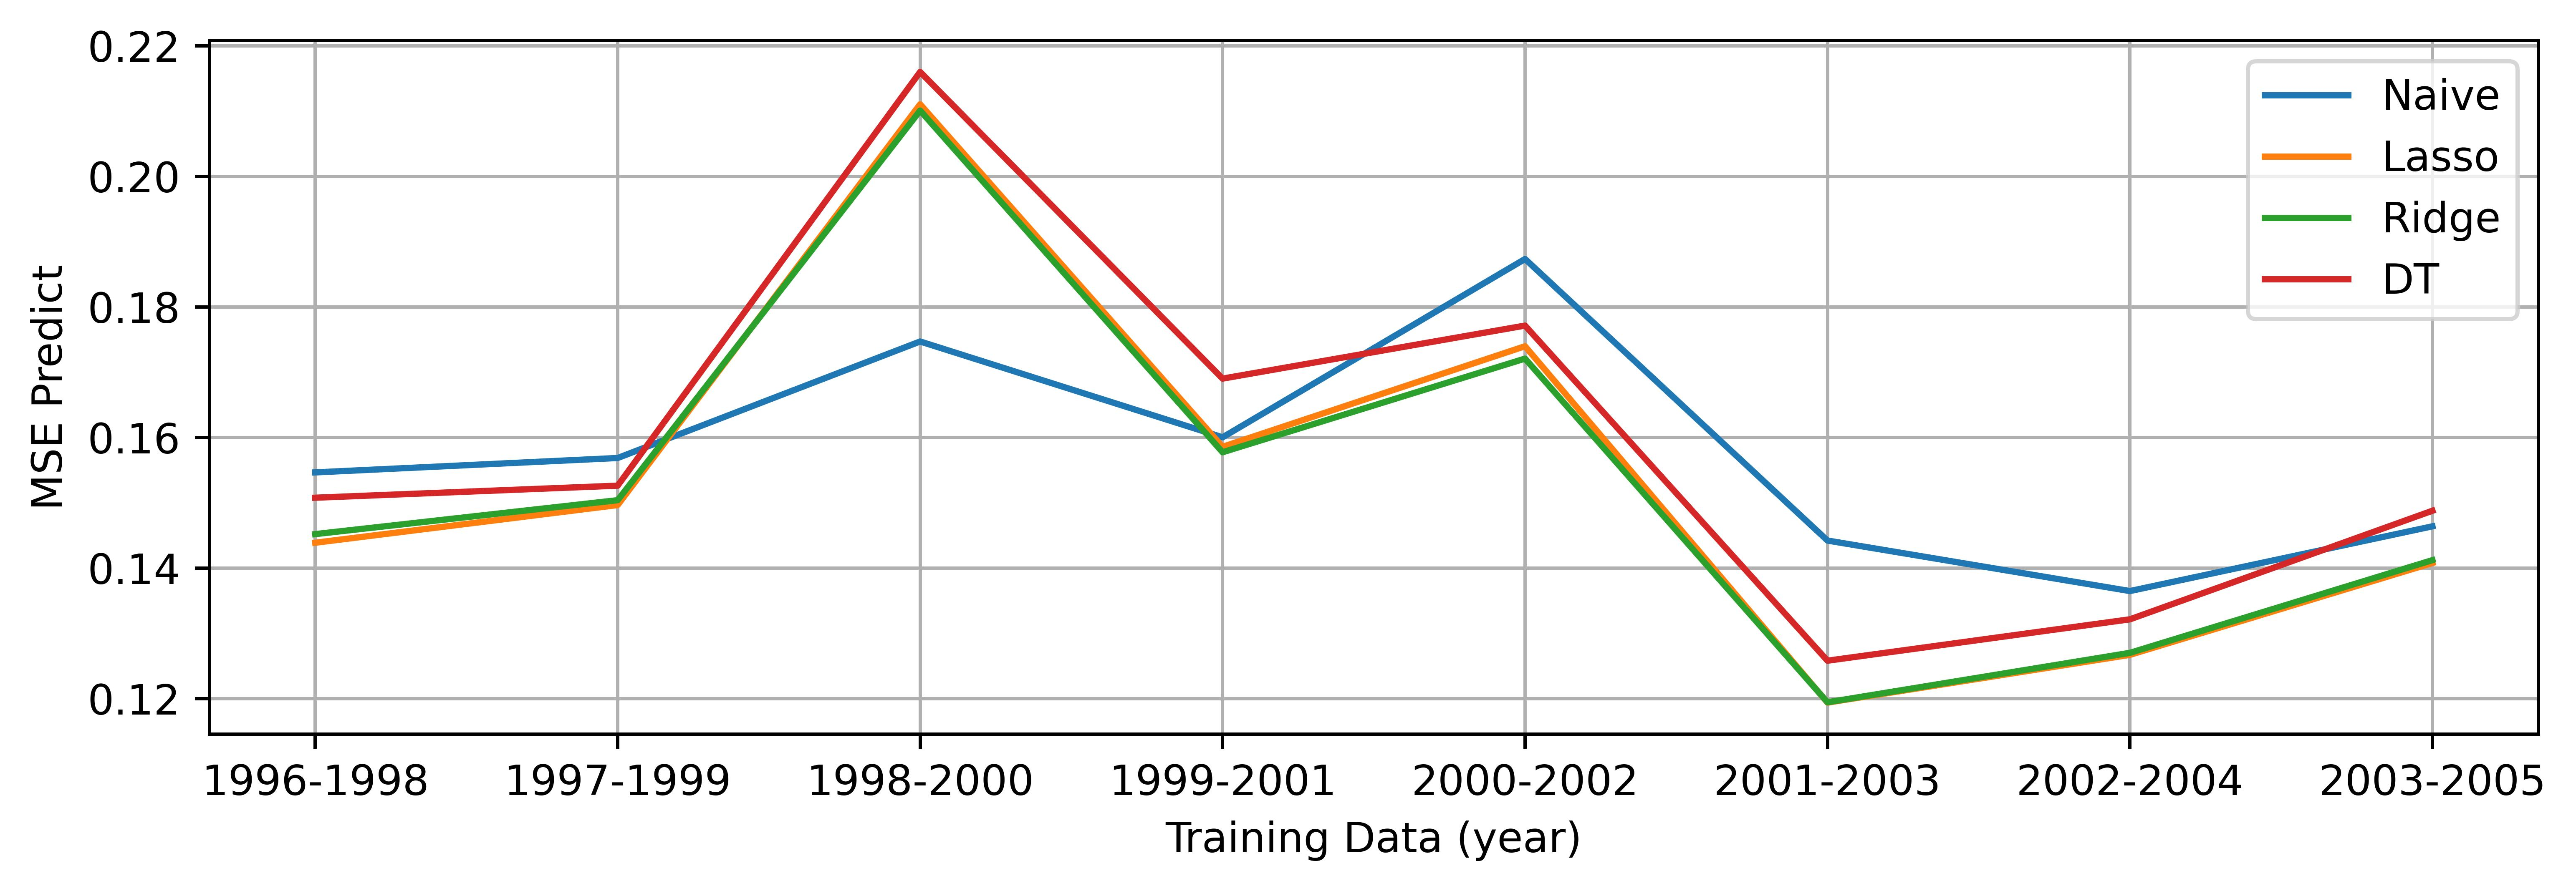
\includegraphics[width=0.7\textwidth]{../Result/Res-3_MSE_pred.jpg}
    \caption{MAE and MSE for predicting the following 1-year's data with the model trained by the previous 3-years' data.}
    \label{figure-3-year-pred}
  \end{figure}
  \clearpage
}

Similar to the result of 1-year's training data, the result still shows the influence of the dot-com bubble and the Sarbanes-Oxley Act. Meanwhile, the errors of three models become more closer and more prediction are better than or equivalent to the Naive model, which implies the higher stability and higher accuracy than the model based on the 1-year's data.

\subsection{Wrod Features}

Another problem we concern about is the words feature, especially the difference and similarly across years or models. Thus we compare the words features given by different models with training data from different years. The Table \ref{table-words-feature-year} compares the words features across years, where the column ``Increasing Common" and ``Decreasing Common" shows the rate of the nearby two years' common features related to the increasing or decreasing volatility, and the column ``Different" shows the rate of the features that are corresponding to the different trend, i.e. the rate of the features that changes the meanings in two years.

\afterpage{
  \clearpage
  \begin{table}[p]
    \centering
    \begin{tabular}{|c|c|c|c|c|}
      \hline
      Year                       & Method        & Increasing Common          & Decreasing Common          & Different                   \\
      \hline
      \multirow{3}{*}{1996-1997} & Lasso         & $53.9\%$                   & $60.6\%$                   & $1.9\%$                     \\
      \cline{2-5}
                                 & Ridge         & $48.3\%$                   & $55.1\%$                   & $2.9\%$                     \\
      \cline{2-5}
                                 & Decision Tree & $62.7\%$                   & $15.8\%$                   & $3.6\%$                     \\
      \hline
      \multirow{3}{*}{1997-1998} & Lasso         & $35.1\%$                   & $39.2\%$                   & $6.4\%$                     \\
      \cline{2-5}
                                 & Ridge         & $38.1\%$                   & $36.9\%$                   & $7.55\%$                    \\
      \cline{2-5}
                                 & Decision Tree & $46.2\%$                   & $29.4\%$                   & $6.75\%$                    \\
      \hline
      \multirow{3}{*}{1998-1999} & Lasso         & \textcolor{blue}{$23.6\%$} & $31.7\%$                   & $5.6\%$                     \\
      \cline{2-5}
                                 & Ridge         & \textcolor{blue}{$20.2\%$} & $32.1\%$                   & $8.35\%$                    \\
      \cline{2-5}
                                 & Decision Tree & $37.1\%$                   & $18.8\%$                   & $8.4\%$                     \\
      \hline
      \multirow{3}{*}{1999-2000} & Lasso         & \textcolor{red}{$3.8\%$}   & \textcolor{blue}{$27.8\%$} & \textcolor{blue}{$17.1\%$}  \\
      \cline{2-5}
                                 & Ridge         & \textcolor{red}{$9.9\%$}   & $38.6\%$                   & $6.55\%$                    \\
      \cline{2-5}
                                 & Decision Tree & $29.3\%$                   & $33.2\%$                   & $4.4\%$                     \\
      \hline
      \multirow{3}{*}{2000-2001} & Lasso         & \textcolor{red}{$5.1\%$}   & \textcolor{blue}{$24.9\%$} & $1.2\%$                     \\
      \cline{2-5}
                                 & Ridge         & \textcolor{red}{$13.2\%$}  & \textcolor{blue}{$18.9\%$} & $3.25\%$                    \\
      \cline{2-5}
                                 & Decision Tree & $23.9\%$                   & $32.7\%$                   & $6.2\%$                     \\
      \hline
      \multirow{3}{*}{2001-2002} & Lasso         & $38.0\%$                   & $30.4\%$                   & $2.7\%$                     \\
      \cline{2-5}
                                 & Ridge         & $42.2\%$                   & $35.7\%$                   & $4.15\%$                    \\
      \cline{2-5}
                                 & Decision Tree & $23.7\%$                   & \textcolor{red}{$3.6\%$}   & \textcolor{blue}{$10.9\%$}  \\
      \hline
      \multirow{3}{*}{2002-2003} & Lasso         & $31.7\%$                   & $31.0\%$                   & \textcolor{blue}{$12.15\%$} \\
      \cline{2-5}
                                 & Ridge         & $35.8\%$                   & $36.4\%$                   & $9.2\%$                     \\
      \cline{2-5}
                                 & Decision Tree & $45.7\%$                   & \textcolor{red}{$5.8\%$}   & $4.3\%$                     \\
      \hline
      \multirow{3}{*}{2003-2004} & Lasso         & \textcolor{blue}{$26.2\%$} & \textcolor{blue}{$58.3\%$} & $3.15\%$                    \\
      \cline{2-5}
                                 & Ridge         & \textcolor{blue}{$27.3\%$} & \textcolor{blue}{$44.6\%$} & $1.25\%$                    \\
      \cline{2-5}
                                 & Decision Tree & \textcolor{blue}{$34.7\%$} & \textcolor{red}{$2.0\%$}   & \textcolor{blue}{$11.85\%$} \\
      \hline
      \multirow{3}{*}{2004-2005} & Lasso         & $42.2\%$                   & $38.3\%$                   & $6.4\%$                     \\
      \cline{2-5}
                                 & Ridge         & $45.5\%$                   & $43.6\%$                   & $9.3\%$                     \\
      \cline{2-5}
                                 & Decision Tree & $56.7\%$                   & \textcolor{red}{$7.3\%$}   & $2.1\%$                     \\
      \hline
    \end{tabular}
    \caption{The rate of common and different word features across different years. The column ``Increasing Common" and ``Decreasing Common" shows the rate of the nearby two years' common features related to the increasing or decreasing volatility, the column ``Different" shows the rate of the features that are corresponding to the different trend, i.e. the rate of the features that changes the meanings in two years. Values in red are outliers from the whole, and blue means the large gap from the previous and following year.}
    \label{table-words-feature-year}
  \end{table}
  \clearpage
}

This table shows that in the most of cases, the word features are similar between the nearby years, while there are some abnormal values, mostly around 2000 and 2003. The the abnormal values are corresponding to the year of the dot-com bubble and the Sarbanes-Oxley Act, which confirm the conclusion that the big events will affect the information or the distribution of the wrods, and it also shows that the firm are more likely to follow the act since 2003.

The Table \ref{table-words-feature-model} compares the word features given by different models. Similar to the previous, the rates of the common features and different features shows that the Lasso and Ridge regression shares most of the features, while the decision tree gives the totally different features.

\afterpage{
  \clearpage
  \begin{table}[p]
    \centering
    \begin{tabular}{|c|c|c|c|c|}
      \hline
      Year                  & Compared Methods       & Increasing Common & Decreasing Common & Different \\
      \hline
      \multirow{3}{*}{1996} & Lasso \& Ridge         & $75.2\%$          & $71.6\%$          & $0.15\%$  \\
      \cline{2-5}
                            & Lasso \& Decision Tree & $23.2\%$          & $7.7\%$           & $27.0\%$  \\
      \cline{2-5}
                            & Ridge \& Decision Tree & $36.1\%$          & $25.1\%$          & $17.35\%$ \\
      \hline
      \multirow{3}{*}{1997} & Lasso \& Ridge         & $82.0\%$          & $87.2\%$          & $0.15\%$  \\
      \cline{2-5}
                            & Lasso \& Decision Tree & $15.4\%$          & $7.3\%$           & $25.85\%$ \\
      \cline{2-5}
                            & Ridge \& Decision Tree & $16.6\%$          & $12.2\%$          & $25.6\%$  \\
      \hline
      \multirow{3}{*}{1998} & Lasso \& Ridge         & $84.4\%$          & $85.5\%$          & $0.2\%$   \\
      \cline{2-5}
                            & Lasso \& Decision Tree & $14.1\%$          & $15.1\%$          & $15.4\%$  \\
      \cline{2-5}
                            & Ridge \& Decision Tree & $12.2\%$          & $15.6\%$          & $18.6\%$  \\
      \hline
      \multirow{3}{*}{1999} & Lasso \& Ridge         & $67.9\%$          & $83.9\%$          & $0.35\%$  \\
      \cline{2-5}
                            & Lasso \& Decision Tree & $17.8\%$          & $23.8\%$          & $19.8\%$  \\
      \cline{2-5}
                            & Ridge \& Decision Tree & $11.5\%$          & $23.1\%$          & $24.0\%$  \\
      \hline
      \multirow{3}{*}{2000} & Lasso \& Ridge         & $68.1\%$          & $55.3\%$          & $1.85\%$  \\
      \cline{2-5}
                            & Lasso \& Decision Tree & $19.0\%$          & $25.1\%$          & $17.6\%$  \\
      \cline{2-5}
                            & Ridge \& Decision Tree & $24.1\%$          & $9.5\%$           & $26.1\%$  \\
      \hline
      \multirow{3}{*}{2001} & Lasso \& Ridge         & $91.7\%$          & $92.9\%$          & $0.1\%$   \\
      \cline{2-5}
                            & Lasso \& Decision Tree & $5.5\%$           & $0.9\%$           & $31.55\%$ \\
      \cline{2-5}
                            & Ridge \& Decision Tree & $6.8\%$           & $1.6\%$           & $30.55\%$ \\
      \hline
      \multirow{3}{*}{2002} & Lasso \& Ridge         & $88.6\%$          & $79.1\%$          & $0.1\%$   \\
      \cline{2-5}
                            & Lasso \& Decision Tree & $37.7\%$          & $49.8\%$          & $9.75\%$  \\
      \cline{2-5}
                            & Ridge \& Decision Tree & $33.8\%$          & $39.2\%$          & $14.35\%$ \\
      \hline
      \multirow{3}{*}{2003} & Lasso \& Ridge         & $93.6\%$          & $89.5\%$          & $0.15\%$  \\
      \cline{2-5}
                            & Lasso \& Decision Tree & $13.4\%$          & $10.4\%$          & $27.05\%$ \\
      \cline{2-5}
                            & Ridge \& Decision Tree & $15.2\%$          & $13.9\%$          & $25.45\%$ \\
      \hline
      \multirow{3}{*}{2004} & Lasso \& Ridge         & $75.2\%$          & $73.4\%$          & $0.2\%$   \\
      \cline{2-5}
                            & Lasso \& Decision Tree & $23.5\%$          & $24.2\%$          & $21.25\%$ \\
      \cline{2-5}
                            & Ridge \& Decision Tree & $30.4\%$          & $20.4\%$          & $20.85\%$ \\
      \hline
      \multirow{3}{*}{2005} & Lasso \& Ridge         & $95.6\%$          & $90.8\%$          & $0.4\%$   \\
      \cline{2-5}
                            & Lasso \& Decision Tree & $9.9\%$           & $2.5\%$           & $27.5\%$  \\
      \cline{2-5}
                            & Ridge \& Decision Tree & $10.2\%$          & $5.2\%$           & $28.7\%$  \\
      \hline
    \end{tabular}
    \caption{The rate of common and different word features across different models. The column ``Increasing Common" and ``Decreasing Common" shows the rate of the nearby two years' common features related to the increasing or decreasing volatility, the column ``Different" shows the rate of the features that are corresponding to the different trend, i.e. the rate of the features that changes the meanings in two years. Values in red are outliers from the whole, and blue means the large gap from the previous and following year.}
    \label{table-words-feature-model}
  \end{table}
}

We try to figure out the reason behind this phenomena by analyse the coefficients  given by the models. The parameter shows that the decisionn tree puts a higher importance on the historical volatility, while the Lasso and Ridge regression gives a much more averagely coefficients. For example, with the training data from 1996, the decision tree gives all the word importance less than $0.1$, while those given by the Lasso and Ridge regression can be up to $0.5$. This might be caused by many reasons, but we believe that the most important one is that the decision tree is in fact non linear, thus when it tries to fit the data, it will obviously concern more on the historical volatility as it will be much more significantly different compare with the word features. One possible way to reduce this is to predict the difference of the volatility, or simply do the classification on the trend, which may improve the preformance in further research.

\section{Conclusion}

We applied the Lasso regression, Ridge regression, and decision tree to the companies' 10-K report, as well as the historical volatility, to forecast the volatility. Similar to the previous research\cite{kogan2009predicting}, our result also shows that the 10-K report, especially the report after the Sarbanes–Oxley Act, can help to predict the value better than the naive model with the similar word features across models and years, and more training data can lead to a better model performance. Furthermore, big events like the dot-com bubble and the Sarbanes-Oxley Act can make a significant effect on the information or the distribution of the text.


\afterpage{
  \clearpage
  \bibliographystyle{unsrt}
  \bibliography{reference.bib}
  \addcontentsline{toc}{section}{References}
  \clearpage
}

\newpage

\appendix
\renewcommand\thesection{\Alph{section}}

\section{Author Contributions}

\begin{itemize}
  \item WANG Zeyu: Write and test the code for processing, Lasso and Ridge regression; Write the Result and Conclusion sections of the report.
  \item LIU Chang: Write and test the code for Decision tree; Write the Method section of the report.
  \item TAN Huangao: Write and test the code for text processing; Write the Method section of the report.
  \item LI Borui: Test the code; Write the Introduction section of the report.
  \item ZHU Xinqi: Write the Introduction section of the report; Make the slide; Do the presentation.
  \item GAO Yifeng: Write the Find section of the report; Make the slide; Do the presentation.
\end{itemize}

\end{document}